\setlength{\columnsep}{3pt}
\begin{flushleft}
	
	\paragraph{What is an MBR?}
	\begin{itemize}
		\item MBR stands for \textbf{Master Boot Recorder}.
		\item MBR is the first \textbf{512 bytes} of HDD.
		\item MBR consists of:
		\begin{itemize}
			\item Bootloader (446 bytes in size) - More on this in chapter 17 under section 17.1.4.
			\item \textbf{Partition Table}  (64 bytes in size) - Stores entry of maximum 4 partitions (16 byte entry for each partition).
			\item Magic number (2 bytes in size) - More on this in chapter 17 under section 17.1.3.
		\end{itemize}
	\end{itemize}	
	 
	
		\begin{figure}[h!]
			\centering
			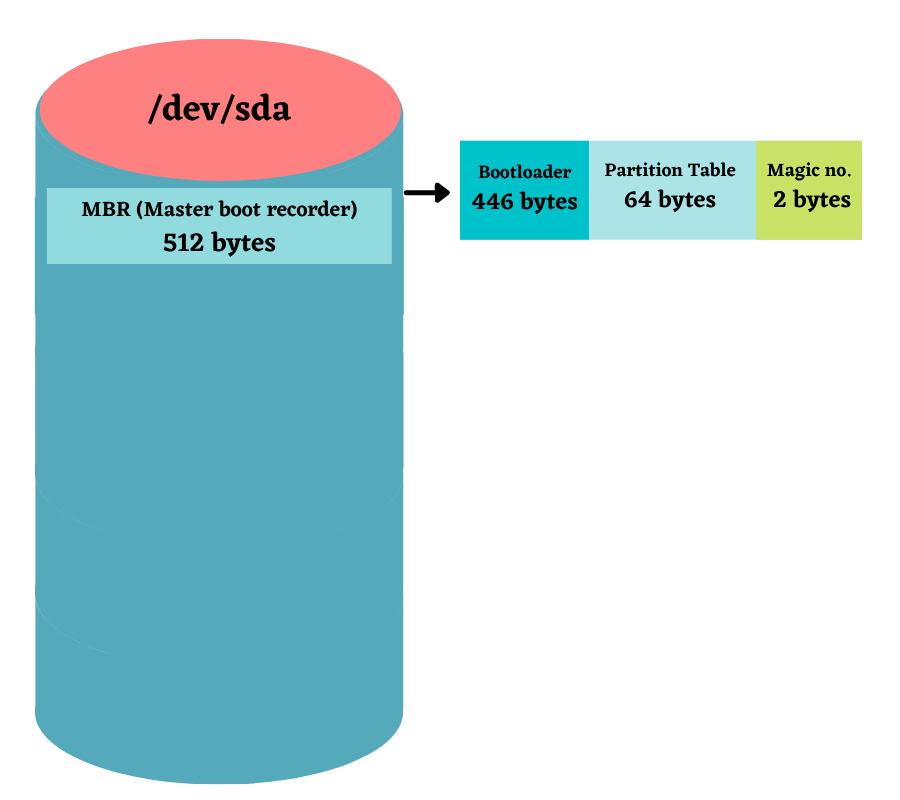
\includegraphics[scale=.6]{content/chapter8/images/correction3.png}
			\caption{MBR}
			\label{mbr_naming}
		\end{figure}		
	
\end{flushleft}

\newpage

